

\tikzset{every picture/.style={line width=0.75pt}} %set default line width to 0.75pt        

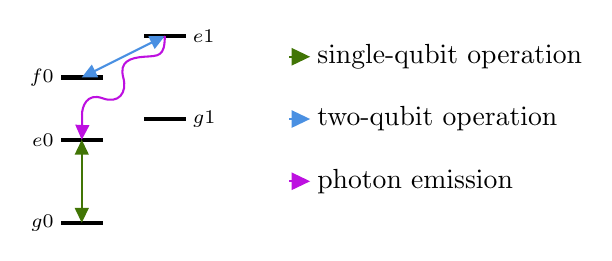
\begin{tikzpicture}[x=0.75pt,y=0.75pt,yscale=-1,xscale=1]
%uncomment if require: \path (0,300); %set diagram left start at 0, and has height of 300

%Straight Lines [id:da9036150792074441] 
\draw [line width=1.5]    (100,100) -- (120,100) ;
%Straight Lines [id:da3892496668455091] 
\draw [line width=1.5]    (140,80) -- (160,80) ;
%Straight Lines [id:da8780144362496497] 
\draw [line width=1.5]    (100,130) -- (120,130) ;
%Straight Lines [id:da9845944648914766] 
\draw [line width=1.5]    (100,170) -- (120,170) ;
%Straight Lines [id:da40423833166537637] 
\draw [line width=1.5]    (140,120) -- (160,120) ;
%Straight Lines [id:da9138884186505395] 
\draw [color={rgb, 255:red, 65; green, 117; blue, 5 }  ,draw opacity=1 ]   (110,133) -- (110,167) ;
\draw [shift={(110,170)}, rotate = 270] [fill={rgb, 255:red, 65; green, 117; blue, 5 }  ,fill opacity=1 ][line width=0.08]  [draw opacity=0] (7.14,-3.43) -- (0,0) -- (7.14,3.43) -- cycle    ;
\draw [shift={(110,130)}, rotate = 90] [fill={rgb, 255:red, 65; green, 117; blue, 5 }  ,fill opacity=1 ][line width=0.08]  [draw opacity=0] (7.14,-3.43) -- (0,0) -- (7.14,3.43) -- cycle    ;
%Straight Lines [id:da18399826038705747] 
\draw [color={rgb, 255:red, 74; green, 144; blue, 226 }  ,draw opacity=1 ]   (147.32,81.34) -- (112.68,98.66) ;
\draw [shift={(110,100)}, rotate = 333.43] [fill={rgb, 255:red, 74; green, 144; blue, 226 }  ,fill opacity=1 ][line width=0.08]  [draw opacity=0] (7.14,-3.43) -- (0,0) -- (7.14,3.43) -- cycle    ;
\draw [shift={(150,80)}, rotate = 153.43] [fill={rgb, 255:red, 74; green, 144; blue, 226 }  ,fill opacity=1 ][line width=0.08]  [draw opacity=0] (7.14,-3.43) -- (0,0) -- (7.14,3.43) -- cycle    ;
%Straight Lines [id:da14000382288661184] 
\draw [color={rgb, 255:red, 65; green, 117; blue, 5 }  ,draw opacity=1 ]   (210,90) -- (217,90) ;
\draw [shift={(220,90)}, rotate = 180] [fill={rgb, 255:red, 65; green, 117; blue, 5 }  ,fill opacity=1 ][line width=0.08]  [draw opacity=0] (8.93,-4.29) -- (0,0) -- (8.93,4.29) -- cycle    ;
%Straight Lines [id:da9331304771806838] 
\draw [color={rgb, 255:red, 74; green, 144; blue, 226 }  ,draw opacity=1 ]   (210,120) -- (217,120) ;
\draw [shift={(220,120)}, rotate = 180] [fill={rgb, 255:red, 74; green, 144; blue, 226 }  ,fill opacity=1 ][line width=0.08]  [draw opacity=0] (8.93,-4.29) -- (0,0) -- (8.93,4.29) -- cycle    ;
%Curve Lines [id:da6855478455179863] 
\draw [color={rgb, 255:red, 189; green, 16; blue, 224 }  ,draw opacity=1 ]   (150,80) .. controls (150,90.17) and (147,89.5) .. (140,90) .. controls (133,90.5) and (128,92.5) .. (130,100) .. controls (132,107.5) and (127.67,112.83) .. (120,110) .. controls (112.33,107.17) and (110.08,114.29) .. (110.13,117.88) .. controls (110.16,120.62) and (110.16,123.77) .. (110.09,127.01) ;
\draw [shift={(110,130)}, rotate = 272.25] [fill={rgb, 255:red, 189; green, 16; blue, 224 }  ,fill opacity=1 ][line width=0.08]  [draw opacity=0] (7.14,-3.43) -- (0,0) -- (7.14,3.43) -- cycle    ;
%Straight Lines [id:da22870453087792075] 
\draw [color={rgb, 255:red, 189; green, 16; blue, 224 }  ,draw opacity=1 ]   (210,150) -- (217,150) ;
\draw [shift={(220,150)}, rotate = 180] [fill={rgb, 255:red, 189; green, 16; blue, 224 }  ,fill opacity=1 ][line width=0.08]  [draw opacity=0] (8.93,-4.29) -- (0,0) -- (8.93,4.29) -- cycle    ;

% Text Node
\draw (98,100) node [anchor=east] [inner sep=0.75pt]  [font=\scriptsize]  {$f0$};
% Text Node
\draw (98,130) node [anchor=east] [inner sep=0.75pt]  [font=\scriptsize]  {$e0$};
% Text Node
\draw (98,170) node [anchor=east] [inner sep=0.75pt]  [font=\scriptsize]  {$g0$};
% Text Node
\draw (162,80) node [anchor=west] [inner sep=0.75pt]  [font=\scriptsize]  {$e1$};
% Text Node
\draw (162,120) node [anchor=west] [inner sep=0.75pt]  [font=\scriptsize]  {$g1$};
% Text Node
\draw (222,90) node [anchor=west] [inner sep=0.75pt]   [align=left] {single-qubit operation};
% Text Node
\draw (222,120) node [anchor=west] [inner sep=0.75pt]   [align=left] {two-qubit operation};
% Text Node
\draw (222,150) node [anchor=west] [inner sep=0.75pt]   [align=left] {photon emission};


\end{tikzpicture}